\section[تمرین دوم - سؤال سوم: بررسی نفرین ابعاد]
{\faProjectDiagram\ \ تمرین دوم ـ سؤال سوم: بررسی پدیده نفرین ابعاد (\lr{Curse of Dimensionality})}

\begin{stepbox}

\field{هدف و معرفی مسئله}{
هدف این بخش، بررسی تجربی یکی از چالش‌های بنیادین در یادگیری ماشین و پردازش داده تحت عنوان **نفرین ابعاد (\lr{Curse of Dimensionality})** است. 

با افزایش ابعاد داده‌ها، فضای حالت به قدری بزرگ و خلوت (\lr{Sparse}) می‌شود که محاسبات مبتنی بر فاصله (نظیر \lr{k-NN} یا خوشه‌بندی) دچار اختلال شدید شده و مفهوم «همسایگی نزدیک» معنای فیزیکی و آماری خود را از دست می‌دهد.
}

\field{نحوه پیاده‌سازی و فرمول محاسباتی}{
برای بررسی این پدیده، در هر بعد $d$ از ۲ تا ۵۰ ($d \in [2, 50]$) دو بردار تصادفی $x$ و $y$ با درایه‌های تصادفی صحیح در بازه $[0, 100]$ با استفاده از تابع \lr{\texttt{np.random.randint}} ایجاد گردید. سپس فاصله اقلیدسی بین آن‌ها به صورت زیر محاسبه شد:

\[
D(x, y) = \|x - y\|_2 = \sqrt{\sum_{i=1}^{d} (x_i - y_i)^2}
\]
}

\field{نمودار و تحلیل خروجی}{
نمودار زیر تغییرات فاصله اقلیدسی دو بردار تصادفی را بر حسب افزایش ابعاد از $d=2$ تا $d=50$ نشان می‌دهد:

\vspace{0.4cm}

\begin{center}
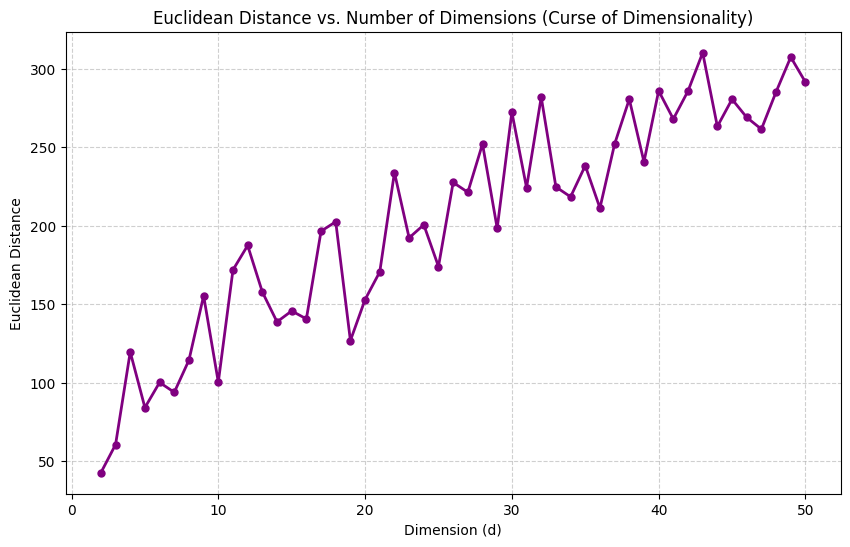
\includegraphics[width=.82\textwidth]{images/curse_of_dimensionality.png}
\captionof{figure}{تغییرات فاصله اقلیدسی بر حسب تعداد ابعاد ($d$)}
\label{fig:curse_dim}
\end{center}

\begin{itemize}
\item **روند صعودی فاصله اقلیدسی:** همان‌طور که در نمودار مشخص است، با افزایش ابعاد $d$، میانگین فاصله اقلیدسی بین دو نقطه تصادفی به شدت رشد کرده و از حدود $40$ در فضای ۲بعدی به بیش از $290$ در فضای ۵۰بعدی می‌رسد.
\item **علت ریاضی:** هر بعد جدید، یک جمله مثبت $(x_i - y_i)^2$ به زیر رادیکال اضافه می‌کند که باعث افزایش مجموع مربع خطاهایت تحت جذر می‌شود.
\end{itemize}
}

\field{استنباط و نتیجه‌گیری}{
تحلیل این خروجی، مفاهیم زیر را در یادگیری ماشین روشن می‌سازد:

\begin{enumerate}
\item **دور شدن نقاط از یکدیگر در ابعاد بالا:** در فضاهای با ابعاد بسیار بالا، تمامی نقاط به طرز عجیبی از هم دور شده و فاصله‌های نسبی بین تمام جفت‌نقاط تقریباً یکسان می‌گردد.
\item **ضرورت الگوریتم‌های کاهش بعد:** همین پدیده نشان می‌دهد چرا در داده‌های واقعی با ابعاد بالا، استفاده از روش‌هایی مانند \lr{PCA} و \lr{LDA} قبل از اعمال الگوریتم‌های یادگیری حیاتی و ضروری است.
\end{enumerate}
}

\end{stepbox}